\documentclass{article}
\usepackage[utf8]{inputenc}

\title{Literature Review}
\author{Christopher MacKinnon }
\date{November 2020}



\usepackage[
style=ieee,
sorting=ynt,
backend=biber
]{biblatex}

\addbibresource{references.bib} %Imports bibliography file


\usepackage{graphicx,amsmath,bm}

\begin{document}



\maketitle

%INTRO
	%Introduction and problem definition for Hyperparameters and Hyperparameter Search
	\section{Hyper-Parameters}

		Hyper-parameter optimisation is traditionally considered a noisy, black-box optimisation problem. A manual search combing a grid search and expert knowledge has been the standard approach to this problem in the past. It was shown that a random search could perform as well as, or better than, grid search in the same time \cite{50}. This type of search has become a minimum benchmark or starting point for many hyper-parameter optimisation techniques. \cite{39}\cite{48} Recently, taking advantage of the increase in parallel and cloud computing power has become a key aspect of these systems, requiring robust methods that can operate efficiently at scale. Hyper-parameters can contain continuous, discrete and categorical variables requiring flexible approaches to find optimal solutions across a wide range of architectures and algorithms. 



	%Closer look at the specific issues linked to Architecture search and NAS i.e. graphs, cells
	\section {Architecture Search}

		There has been an increase in interest in Neural Architecture Search (NAS) recently as these methods began to outperform human designed models. \cite{51}\cite{41} These systems are able to design at scale creating intricate topologies for large, deep neural networks (DNN), while discovering novel variants in the components used to build these networks. \cite{25} \cite{4}



		%%%Micro vs macro 
		
		%%%Refinement of search space over time




\section {Genetic Algorithms}

	Genetic algorithms borrow optimisation strategies from those found in nature. One of the main benefits of genetic algorithms is the flexibility in terms of categorical, discrete and continuous variables. GAs are naturally suited to the creation of novel topologies\cite{24} \cite{25}, and can often produce targeted architectures that deviate from the generalised templates that commonly used due to their effectiveness across a range of domains. GAs have also been used on a more granular level, creating novel variants of network components suited to a specific task \cite{25}


	\subsection{Crossover and Genetic Encoding}

		Crossover is the recombination of two successful networks into a “child” network which is common to many GA approaches to NAS. \cite{3}\cite{24}\cite{5} This can be implemented through a wide variety of mechanisms based on the network encoding method which is used. Ablation tests on GA systems have shown that while crossover can result in an overall improvement if carried out correctly, it can often be far less significant that other aspects of GA. \cite{5}\cite{24}

		\par

		One of the core components to GA is the genetic encoding of model architectures. This is an important aspect of a successful GA due to the reliance of crossover on this representation of the network to carry meaningful aspects of the models forward. \cite{24} Another issue that is important to consider when designing a genetic encoding methods is the problem of competing conventions or the permutation problem\cite{38}\cite{24}. In the context of ANNs this refers to a scenario where the same architecture can be represented by multiple encodings. This can lead to inefficient allocation of computational resources and irregularities during crossover operations. \cite{24}


	\subsection{NEAT}


		NeuroEvolution of Augmenting Topologies (NEAT) \cite{24} describes a framework for evolving neural networks which addresses many of the issues faced by GA, such as a formalised system for crossover, genetic encoding, the permutation problem and the protection of innovation. NEATs success is limited to smaller networks, however, there have been several extensions to NEAT, adapting it for larger, deeper networks. \cite{44}\cite{25}

		NEAT makes use of an innovation number which denotes the order in which mutations occurred to the network. This enables a matching of connections or nodes in the crossover process between networks giving the method a structured process. Speciation is a component of GA which separates models based on genetic distance into subcategories. This protects innovation allowing solutions to be explored and reach maturity without competing with the wider population. In practice this creates a less greedy algorithm supporting a greater diversity of solutions and, in theory, improving performance on multi-modal functions. 

		Ablation testing was able to show the dependence of the wider system on each of these components. Speciation was shown to offer a very significant contribution to overall success of the method, while aspects such as crossover was shown to have a much smaller, but still statically significant, improvements in performance.


	\subsection{CoDeepNEAT}

		CoDeepNEAT \cite{25} is an expansion to NEAT for use with deep neural networks. This approach was able to achieve near parity with SOTA on CIFAR-10 as well as image captioning benchmarks. 

		\par
		CoDeepNEAT is based on a bi-level optimisation approach to the CASH problem, implementing a hierarchical approach in which “blueprints” and modules are evolved independently. A blueprint is a graph of nodes which are replaced with modules to create complete networks for evaluation. The fitness score of a network is applied to both the blueprint and the modules, with the module score being an average of all the networks which contained the blueprint. This method was also applied to LSTM networks, which was able to produce an LSTM variant which outperform the standard LSTM cell.


	\subsection{N-Level Hierarchical Representation }

		\cite{4} introduced a nested system for NAS which expands upon the method described in \cite{25} from a bi-level hierarchy to an Nnlevel hierarchy. In this system, primitive operations (i.e. convolutional cells, linear cells) are considered level one. level two representations are a set of graph structures combining these lower level cells. These second level representations are then combined replacing the nodes in a graph to create higher level representation. 


	\subsection{Population Based Training}

		\cite{39} introduced a form of GA which takes inspiration from bandit problems called Population Based Training (PBT). This was able to outperform human tuned networks on reinforcement learning and imagine classification tasks.
		\par
		This is a system for hyper-parameter optimisation which utilizes a variant of the  successive-halving\cite{45} method used in Hyperband (see Sec 4.1) for early-stopping, A portion of the population abandon their search and copy the structure, hyper-parameters and weights of high performing networks. The hyper-parameters of this new replicated network are then mutated randomly to allow for more thorough examination of lucrative search spaces. \cite{13} introduces a similar system targeted at Neural Architecture Search (NAS).
		This method of exploiting successful networks has the additional advantage of producing hyper-parameter schedules that vary over the training process.


	\subsection{LEMONADE}

		\cite{13} approach the problem of NAS with a multi-objective based method that seeks to retain network function across generations via Lamarckian inheritance.
		 For applications in embedded systems or other computational limited environments, the complexity of the network can be an important factor. This system utilizes a Pareto front in the selection process to select a curve of models based on performance and complexity. 
	 

	\subsection{NSGA-NET}

		NSGA-Net \cite{5} is a GA based multi-objective optimisation system for NAS which is build upon NSGA-II\cite{42} and incorporates Bayesian Optimisation methods. This approach was able to achieve parity with SOTA on the CIFAR-10 data-set compared with other NAS solutions (in particular RL based methods) at a significantly lower computational cost using a similar multi-objective method as \cite{13}.

		This approach encodes a group of nodes (a single computational unit, i.e. convolution, pooling in this particular application) as binary strings, these are describes as phases, which are then stacked to describe an entire model. Mutations are applied through bit-flipping of this encoding. Crossover was achieved through a comparison of binary strings where common bits from both parents are retained and unique bits are chosen at random from either parent.

		The final stage of this technique involves applying a Bayesian Network to exploit the phases and their ordering in successful networks to probability distributions which are sampled from to create new solutions.


	\subsection{Aging Evolution}

		\cite{42} produces a GA variant in which the population is selected against based upon the “age” of the network. This method was able to set a new SOTA when scaled up on ImageNET.
		This method maintains a population of networks from which a sub-population of size S are selected and evaluated. The highest scoring network is mutated to create a new child network which replaces the oldest model in the population.  




\section {Many-Armed Bandit and Early-Stopping}

	The problem of hyper-parameter optimisation can also be framed as a many armed bandit problem. This approach seeks to find an effective balance between exploration of new hyper-parameter space and exploitation of known, high performing settings.
	\par
	Early-Stopping is based on the assumption that a partially trained models performance will be predictive of its final performance.[32][47] This assumption can, however, become strained in cases where the variance in convergence time of a set of models is very large. One of the limitation of this method is the final performance with a larger computational budget. This has lead to the incorporation of bandit based strategies into Bayesian and Evolutionary techniques to improve the anytime performance as well as allowing for greater exploration. [32][47][39]


	\subsection{HyperBand}

		Hyperband \cite{48} is an popular example of this strategy and has shown the effectiveness of this method, in particular with respect to anytime performance. Hyperband was able to achieve a reduction in training time of an order of magnitude over Bayesian methods while maintaining only a minor reduction in performance.

		Hyperband can be considered a resource allocation algorithm for Successive-Halving \cite{45}, attacking the problem of balancing the resources allocated to the training of each model (n) with the total number of models trained for a fixed resource budget. Due to the variance of model convergence time between different algorithms or problem domains, this cannot be a static, fit all value. Hyperband effectively performs a grid search of values for n, running a sequence of tests for different values of n within a bounded range.


	\subsection{ASHA}

		Asynchronous Successive Halving Algorithm (ASHA) \cite{34} is a parallelisation technique for the Successive-Halving algorithm. This method has been shown to perform as well as or better than other techniques that incorporate early stopping such as PBT, BOHB and Hyperband on a variety of hyper-parameter optimisation and NAS benchmarks.




\section {Bayesian Optimisation}

	Bayesian Optimisation (BO) methods for hyper-parameter optimisation have become popular over the last decade due to the SOTA performance they can produce \cite{32} \cite{20}. One of the core weaknesses of many BO implementations is the lack of scalability, with models such as Gaussian Processes computationally scaling cubically with observations.
	\par

	The objective of BO and SMBO in general, in the context of hyper-parameter optimisation, can be described as trying to find \(x^* = argmin~ f(x)\) where \(x \in X\) and \(X \subseteq \mathbf{R} ^k\), \textit{X} is a bounded and compact region and \textit{k} is the dimensionality of the search space in our case the number of hyper-parameters. These methods assume correlation between observations and endeavour to use all of the available information to produce useful points for evaluating, \textit{x}, by exploiting a model constructed based upon a set of function query, observations pairs \( D = \{(x_n,y_n)\}_{n=1}^N\) where \(y_n \sim \mathcal{N}(f(x), \sigma_n^2) \).




	\subsection{Posterior Model}

		A posterior model uses the observation history \textit{D} often in combination with some prior to make estimation about the function \textit{f}. These models generally model the value of \textit{f} across the input space, either directly or indirectly, while also having some measure of uncertainty.




		\subsubsection{Gaussian Process}

			The most common model used in hyper-parameter optimisation is a Gaussian Process (GP)\cite{17}. The Gaussian process is non-parametric model which is widely used due to its flexibility and simplicity, allowing many common acquisition functions to be described in a closed form, while having a well calibrated measure of uncertainty.
			\par
			A GP can be considered a generalisation of a multivariate Gaussian distribution to an infinite number of variables. In our case this denotes all possible values within the bounded region \textit{X}. A Gaussian process is fully defined, analogously to a Gaussian distribution, by a mean, \(m(x)\) and covariance function \(K(x,x')\), it is common to use \(m(x) = 0\) as the Gaussian process is generally robust to the mean function given sufficient data.

			\begin{equation}f(x) \sim  \mathcal{N}(m(x) , K(x,x'))\end{equation}
			\begin{equation}f(x) \sim  \mathcal{N}(0 , K(x,x'))\end{equation}

			The covariance function or kernel function is used to generate the covariance matrices in a GP. The kernel is responsible for how both the prior and posterior are expressed. The most commonly used kernel function is the \textit{Squared Exponential Kernel}. The covariance between two points is a function of their separation and a hyper-parameter \textit{l}. 

			\begin{equation}K(x,x') = \sigma^2 exp\left(-\frac{\mathopen|x - x'\mathclose|^2}{2l^2}\right)\end{equation}

			\begin{equation} \label{eq:ncov} K(x,x') = \sigma^2 exp\left(\sum_{i=1}^k-\frac{\mathopen|x_i - x_i'\mathclose|^2}{2l_i^2}\right)\end{equation}

			\begin{equation}\label{eq:sigy} \Sigma(x,x') = K(x,x') + I \sigma_y \end{equation}


			 equation \ref{eq:ncov} shows the kernel function extended to multidimensional problem. for k dimensions there are k+3 hyper-parameters. \textit{l} is the scale length, effectively how quickly the correlation between two points decays or the horizontal scaling for each dimension. \(\sigma\) is the or the vertical scaling. \(\sigma_y\), shown in equation \ref{eq:sigy}, is a representation of noise in the evaluations, this maintains some uncertainty around evaluation points.  In hyper-parameter optimisation and other applications with noisy evaluations, Gaussian noise is added to the covariance matrix to avoid over-fitting. These hyper-parameters have a significant effect of the expression of the model and can be key to the final result, in particular \textit{l}. Because of this, these settings are normally dealt with automatically rather than hand tuned. One approach used in \cite{17} is to integrate over the hyper-parameters using Monte Carlo estimates, however this can be computationally expensive. Another common approach is to use a marginal likelihood estimates and optimise these settings via gradient descent.

 


			\begin{equation}\label{eq:gp1} p(f|\theta,D) = \mathcal{GP}(0,K(x,x'))\end{equation}

			\begin{equation}\label{eq:gp2} p(y|\theta,D) = \mathcal{GP}(0,K(x,x') + I\sigma_y)\end{equation}


 			equations \ref{eq:gp1} and \ref{eq:gp2} show a definition of Gaussian processes over an noiseless and noisy function respectively. For a point of interested, y(x'), the Gaussian process can be considered a joint distribution over the y(x') and the query observation pair history \textit{D}. Using the marginalisation property of gaussians this can be restructured as equation \ref{eq:gp4}. An estimate of \textit{y} at \textit{x'} is simply \textit{y(x')} conditioned on \textit{y(\textbf{x})} 

			\begin{equation}\label{eq:gp4} p(y(\bm{x}),y(x')) \sim \mathcal{N} \left(\begin{pmatrix}
			0\\
			0
			\end{pmatrix},\begin{pmatrix}
			K(\bm{x},\bm{x}}) & K(\bm{x},x')\\
			K(\bm{x},x')^T &  K(x',x')
			\end{pmatrix}\right)\end{equation}

			\begin{equation}\label{eq:inv} p(y(x')|y(\bm{x})) = \frac{p(\bm{x},x')}{p(\bm{x})} \sim  \mathcal{N} (K(\bm{x},x')K(\bm{x},\bm{x}})^{-1}\bm{x},K(x,x) - K(\bm{x},x')K(\bm{x},\bm{x}})^{-1}K(\bm{x},x')^T) \end{equation}


			\begin{equation}p(y(x')|y(\bm{x})) = \frac{p(\bm{x},x')}{p(\bm{x})} \sim  \mathcal{N} (\mu',\sigma') \end{equation}



			\begin{equation}\mu' = K(\bm{x},x')K(\bm{x},\bm{x}})^{-1}\bm{x}\end{equation}

			\begin{equation}\sigma' = K(x,x) - K(\bm{x},x')K(\bm{x},\bm{x}})^{-1}K(\bm{x},x')^T\end{equation}



			Equation \ref{eq:inv} shows the computational issue with Gaussian processes with the inversion of the posterior covariance matrix, \(K(\bm{x},\bm{x})\). This is a \((N,N)\) matrix which means the computational complexity scales cubically \(O(n^3)\) with the number of observations. This issues is further exacerbated in high dimensional search spaces causing GPs to become intractable on large high dimensional problems. Due to the expensive function evaluations in hyper-parameter optimisation, these computational expenses have, until recently, been easily justifiable. However, with the increasing ubiquity of parallel and cloud computing in ML, this limitation has lead to interest in other, more scalable models.


		\subsubsection{Tree-Structured Parzen Estimator}

			The Tree-Structured Parzen Estimator (TPE) is a model introduced by \cite{20} based on Parzen Window Density or Kernel Density estimation. This method was also claimed to outperform both random and GP based Bayesian hyper-parameter optimisation on the MNIST data-set \cite{20}. \cite{32} has more recently used a similar method to great success, leading to its use as the underlying system in the popular Auto-ML tool “HyBandSter” \cite{34}.
			TPE takes an alternative approach to the GP, modelling \(p(x|y)\) and \(p(y)\) rather than \(p(y|x)\) directly. This approach makes use of Kernel Density Estimation (KDE) to build two distribution of hyper-parameter settings which is shown in Figure \ref{fig:tpe1}. equation \ref{eq:TPE} describes the criterion for discriminating between evaluations for division into either \(l(x)\) or \(g(x)\) in a maximization problem. Here \(y*\) is set to be some quantile of the evaluations \(y\) rather than the maximum, this creates two probability distributions one of high performing hyper-parameter combinations and another of lower performing combinations. 

			\begin{equation}\label{eq:TPE} p(x|y) \begin{cases}
									l(x), & \text{if } y>y*\\
									g(x), & \text{if } y\leq y*\end{cases} \end{equation}

			\begin{figure}[h]

			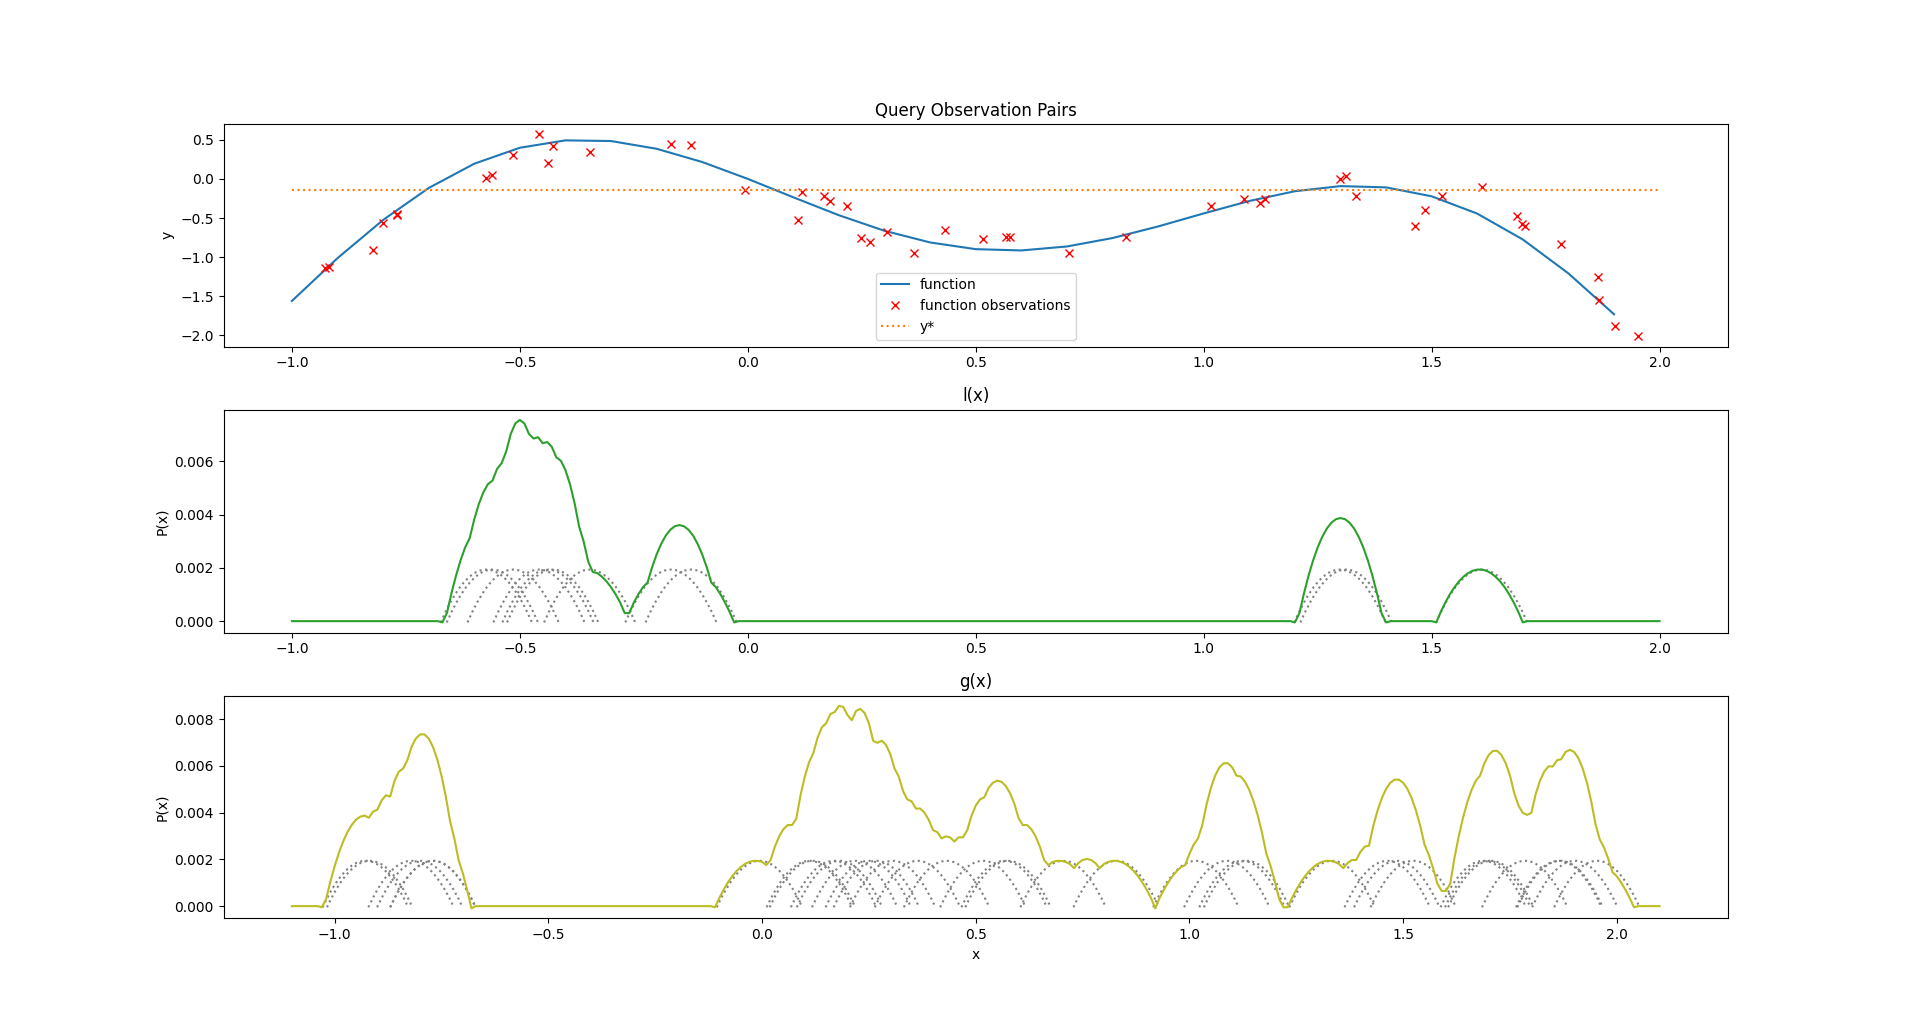
\includegraphics[trim=20 0 0 0 ,scale=0.25]{TPE1.png}

			\caption{Example of the distributions created by KDE during TPE on a 1-dimensional maximisation problem. Top shows noisy observations of a function with y* set so that l(x) contains the upper quartile of evaluation scores. The middle and lower plots show KDE with a Gaussian kernel shown by the dotted lines.}
			\label{fig:tpe1}
			\end{figure}
			Query point acquisition which is discussed in section \ref{AF}, is also simple with TPE. As shown in equation \ref{eq:TPE2}, the ratio of l(x) over g(x) is maximised, this was shown to be equivalent to maximizing EI \cite{20} (Section \ref{EI} ).

			\begin{equation}\label{eq:TPE2} x_{next} = argmax \frac{l(x)}{g(x)}\end{equation}


		\subsubsection{Bayesian Neural Networks}

			Another method for modelling the distribution over a function is with the use of a Bayesian neural network. DNGO \cite{22} is an implementation of this that uses a Deep Neural Network in combination with a Bayesian linear regressor to create an adaptive basis regression to model the posterior. This approach has the advantage of scaling linearly, in terms of computation, with the number of observations rather than cubically as with a GP. This method was able to achieve parity with SOTA in hyper-parameter optimisation on CIFAR-10. BOHAMIANN \cite{40} is another implementation of Bayesian neural networks which was able to out perform DNGO on a number of hyper-parameter optimisation tasks while supporting native parallelisation. 
			\par
			One significant issue with NN based BO methods is the reliance of these techniques on well tuned hyper-parameters of their own to achieve optimal performance. This resulted in DNGO applying the more robust hyper-parameter optimisation system \textit{spearmint} (based on \cite{20}) to the system to optimise its own hyper-parameters.




	\subsection {Acquisition Function} \label{AF}

		The acquisition function is used in BO to select the next query point in hyper-parameter space at which to evaluate, \(x_{next}\), based on the posterior model. This can be considered the criterion against which the latent value of a point in the search space is evaluated. The exploit/explore problem is managed by this component of the system, balancing the use of known high value regions with information gain from areas with large uncertainty. Parallelisation is another important design feature of the acquisition function. Many popular and effective methods are natively sequential in nature and therefore require modification or extension to accommodate parallel query point acquisition. There are asynchronous implementations used as a solution to this problem, which commonly involve updating the posterior model as a worker completes an evaluation, producing a new query point from the updated posterior model and re-dispatching the worker. \cite{26}\cite{27}\cite{20}



		\subsubsection{Expected Improvement / EI-MCMC}\label{EI}

			The most common of acquisition function, in particular when paired with a GP, is Expected Improvement (EI) due to the fact it is considered robust for most problems and does not require complex hyper-parameter tuning of its own. Equation \ref{eq:ei1} defines EI, which can be described as the expectation that a query point \(x\) will improve upon the current best evaluation in the next step, leading to a greedy choice of query points. Equation \ref{eq:ei2} shows how EI can be evaluated in closed form under a GP. From this the framing of the exploration/exploitation problem in terms of \(\Delta_n\) (predicted mean - current best estimate) and predicted variance \(\sigma_n\) can be seen. EI is high when \(\Delta_n\) is large and largest when both  \(\Delta_n\) and \(\sigma_n\) are high, with the former having a much larger effect. The exploration coefficient, \(\xi\), is shown in equation \ref{eq:ei3}. This hyper-parameter limits the greediness of the criterion by devaluing the posterior mean relative to uncertainty, promoting exploration.

			 

			\begin{equation}\label{eq:ei1} EI_n(x) = \mathbf{E} ~max(f(x) -f(x*),0)\end{equation}

			\begin{equation}\label{eq:ei2} EI_n(x) = [\Delta_n(x)]^+ \sigma_n(x)\varphi\left(\frac{\Delta_n(x)}{\sigma_n(x)}\right)  - |\Delta_n(x)| \Phi\left(-\frac{|\Delta_n(x)|}{\sigma_n(x)}\right)\end{equation}

			\begin{equation}\label{eq:ei3}\Delta_n(x) = (\mu(x) - f(x*) - \xi) \end{equation}


			Maximizing EI can be done with a number of approaches. One simplistic approach is simply to perform a grid search over the function. However, one of the beneficial attributes of EI under a GP is the often at least ones differentiable (conditional on the kernel) allowing for gradient descent to be used. it is important to note that EI tends to produce a function which is highly multi-modal, this means in practice gradient descent is restarted from a number of random locations in-order to find the global optimum. Figure \ref{fig:EI1} shows that even in simple problems EI can be multi-modal in nature.
				

			\begin{figure}[h]

			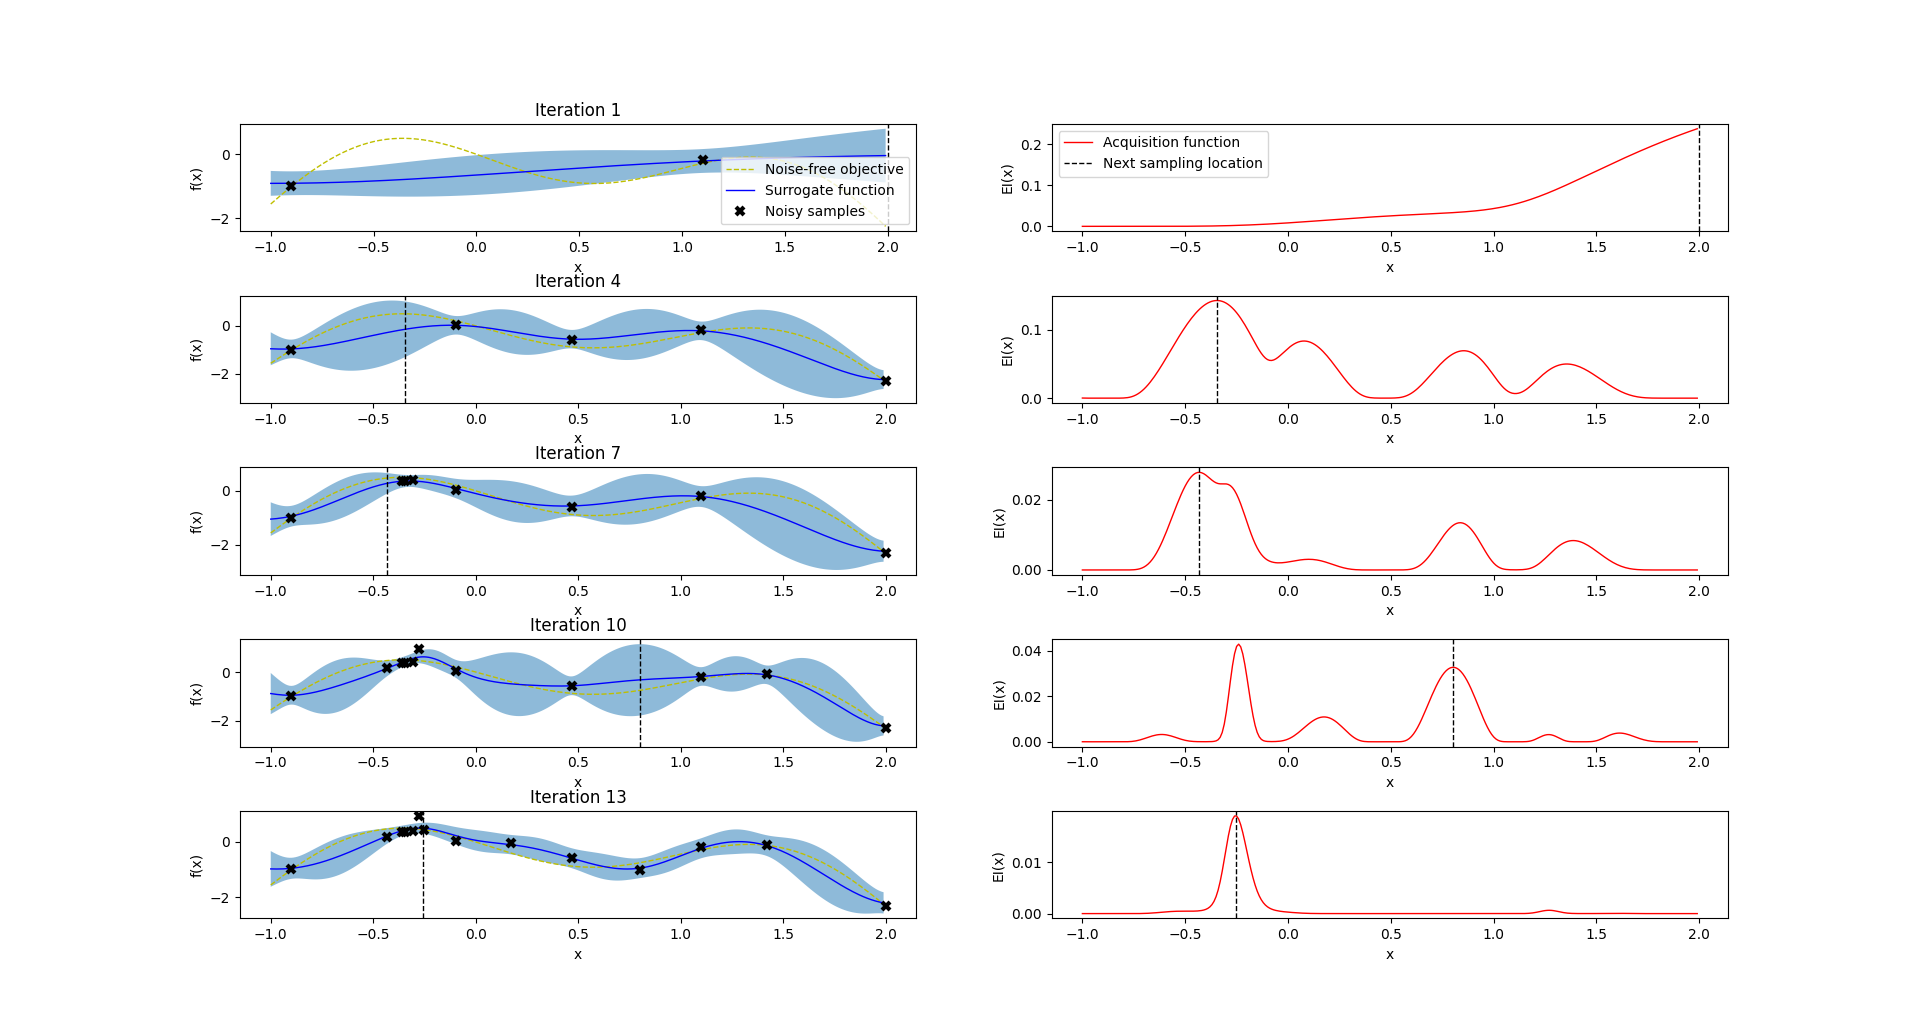
\includegraphics[trim=20 0 0 0 ,scale=0.25]{EIsimp.png}

			\caption{
			Expected improvement optimising a simple one-dimensional problem over a GP for 13 iterations. Left shows the Gaussian process modelling the posterior. Right shows the value curve at selected iterations under the EI criterion.
			}
			\label{fig:EI1}

			\end{figure}



			EI-MCMC is an extension of this function which allows for parallelisation based on Monte Carlo Markov Chain estimates of the acquisition function \cite{17}. In a case where there are a set of \textit{J} points being currently evaluated in parallel, EI cannot simply be re-evaluated on the same posterior as it would produce a redundant evaluation. This approach makes a Monty Carlo estimates via slice sampling at the ongoing evaluation points \({\{x\}}_{j=1}^J\) of the evaluation outcomes, \(\{y\}_{j=1}^J\). One set of these outcomes is referred to as a 'fantasy'. Optimally, EI would be computed across all possible values for \(\{y\}_{j=1}^J\) and the next point selected by integrating over the EI outcomes. In practice this is calculated over a finite number of fantasies with the \(x_{next}\) being the argument maximizing the result of integrating over the acquisition function outputs, described in \ref{eq:EI4}.

			\begin{equation}\label{eq:EI4} x_{next} = argmax~ \widehat{EI}(x; D, \theta,\{x_j\})\end{equation}


		\subsubsection{Upper Confidence Bound}
			Upper Confidence Bound (UCB) is an approach to query point acquisition which is optimisitic towards uncertainty. 

			\begin{equation}\label{eq:UCB1} UBC(x) = \mu(x) + B_n\sigma(x) \end{equation}


			\begin{itemize}

				\item figure

				\item BUCB

				\item scaling factor

				\item guarntee of convergence more robust than EI


		\subsubsection{Local Penalisation}

			One intuitive solution to this problem is the application of local penalization to the acquisition function in order to create batches of query points as shown in \cite{37}. However, this method can be consider as “doubly greedy” \cite{36} in cases where a greedy acquisition function is used as the basis for local penalisation.




		\subsubsection{Thompson Sampling}

			Thompson Sampling (TS) is one method that has been applied to the problem of BO parrallelisation\cite{26}\cite{27}. In TS the next point to be queried (x*) is selected based on a random sampling of the posterior probability distribution. This gives theoretically grounded method for maintaining diversity in synchronise selection of evaluation points without updating the posterior distribution. This was able to outperform other parallel BO methods in hyper-parameter optimisation on the CIFAR-10 data-set. 
			\cite{26} builds on the results of \cite{27} introduction a variant referred to as AEGiS which has a chance of performing a purely explorative evaluation rather than utilising TS.

			 \cite{36} puts forward a non greedy method for the parallel acquisition of query points which was able to outperform other (greedy) parallel BO systems on synthetic and real world bench-marking functions.




\section{Reinforcement Learning}

    Short description of reinforcement learning 
    Pros:
        Strong performance with high enough computational budget
        Incorporates meta-learning, moving away from a black-box perspective
    Cons:
        Very High computational cost

    1. [50] Brought RL-NAS to the mainstream producing neural architectures that outperformed human designed SOTA on cifar-10, this required 800 gpu days or something idk
  
    \subsection{One-shot Architecture Search}
    2. ENAS [52] was an expansion upon RL-NAS which was able to improve efficiency by over 1000x and achieve slightly improved results. This was done by training a single acyclic graph within which the entire search-space was contained. 
    3. [51] was able to show the importance of dropout in the one-shot method described in [52] 




\section{Bi-Level/Gradient Descent}

	[11] STNs - gradient descent for hyper-parameter optimisation

	[53] Darts - gradient descent for cell architecture search  
    



\section{Meta-Learning}

	Meta-learning has gained traction as a possible path away from the black-box perspective of hyper-parameter optimisation. This involves the application of machine learning to configuration selection. This has been implemented in various forms with success, such as a type of transfer learning in network embedding applications \cite{9}. This has also been implemented as an interface which allows experts to effectively warm start an auto-ML pipeline with knowledge of effective configurations for similarly structured problems\cite{29}. Another approach has been to train an agent via reinforcement learning to select configurations[28]. These applications of meta-learning are effective at reducing the convergence time however, rarely achieve significantly superior final performance than the methods they are supplementing.\cite{31}\cite{29}

``


\section{Research Opportunities}

	one-shot/hypernetwork applied to GAs or BO



\printbibliography{}

\end{document}
